\documentclass[aspectratio=169]{beamer}

% Theme selection
\usetheme{Madrid}
\usecolortheme{whale}

% Packages
\usepackage{graphicx}
\usepackage{booktabs}
\usepackage{tikz}
\usetikzlibrary{shapes, positioning, shadows, arrows.meta}
\usepackage{amsmath}
\usepackage{hyperref}
\usepackage{listings}

% Custom Colors
\definecolor{sharifblue}{RGB}{0, 50, 100}
\definecolor{medgreen}{RGB}{40, 140, 40}
\definecolor{alertred}{RGB}{180, 20, 20}
\definecolor{darkred}{RGB}{220, 20, 20}
\setbeamercolor{structure}{fg=sharifblue}
\setbeamercolor{frametitle}{bg=sharifblue, fg=white}

% Title Info
\title[Radiology VLMs]{Vision-Language Models in Radiology}
\subtitle{Zero-Shot Classification, Cross-Modal Retrieval, and Factual Report Generation}
\author[Salehi, Salesi, Daneshgar, Beyrami]{Shayan Salehi, Ali Salesi, Sina Daneshgar, Sina Beyrami}
\institute[SUT]{
  Department of Computer Engineering\\
  Sharif University of Technology
}
\date{February 2026}

\begin{document}

%--- Slide 1: Title ---
\begin{frame}
  \titlepage
\end{frame}

%--- Slide 2: Outline ---
\begin{frame}{Outline}
  \tableofcontents
\end{frame}

\section{Introduction \& Problem Statement}

%--- Slide 3: Problem Statement ---
\begin{frame}{The "Safety Gap" in AI-Driven Radiology}
  
  \begin{columns}
    \column{0.5\textwidth}
    \textbf{The Challenges}
    \begin{itemize}
      \item Radiologists are overworked; AI could help, but...
      \item Current models generate fluent reports with \textcolor{alertred}{\textbf{hidden hallucinations}}
      \item Models output \textcolor{alertred}{\textbf{untrustworthy confidence}} — they don't know when they're wrong
      \item Domain shifts between hospitals cause \textcolor{alertred}{\textbf{performance collapse}}
    \end{itemize}
    
    \column{0.5\textwidth}
    \textbf{Concrete Example: Clinical Hallucination}
    
    \vspace{0.3cm}
    \textit{Patient's chest X-ray shows:} Cardiomegaly (enlarged heart)
    
    \vspace{0.2cm}
    \small
    \fcolorbox{alertred}{white}{
      \parbox{0.45\textwidth}{
        \textbf{Baseline Model Output:}\\
        ``The heart is normal in size\ldots''\\
        \textcolor{alertred}{WRONG}
      }
    }
    
    \vspace{0.2cm}
    \fcolorbox{medgreen}{white}{
      \parbox{0.45\textwidth}{
        \textbf{Our Model Output:}\\
        ``The heart is enlarged\ldots''\\
        \textcolor{medgreen}{CORRECT}
      }
    }
  \end{columns}
  
\end{frame}

%--- Slide 4: Historical Context ---
\begin{frame}{Two Influential Base Architectures}
  
  \begin{columns}
    \column{0.5\textwidth}
    \textbf{CheXzero (Nature BME 2022)}
    \begin{itemize}
      \item Vision-Language Contrastive Learning
      \item ResNet-50 (images) + BioClinicalBERT (text)
      \item Zero-shot classification: no labeled data needed
      \item Limitation: no report generation
    \end{itemize}
    
    \column{0.5\textwidth}
    \textbf{R2Gen (EMNLP 2020)}
    \begin{itemize}
      \item Transformer-based sequence-to-sequence
      \item ResNet-101 + Relational Memory + Meshed Decoder
      \item Generates full reports via teacher forcing
      \item Limitation: optimized on word-level accuracy, not medical truth
    \end{itemize}
  \end{columns}
  
  \vspace{0.5cm}
  \hrule
  \vspace{0.5cm}
  
  \textbf{Our Strategy:} Preserve both architectures' strengths; inject ``medical common sense'' via Reinforcement Learning + Uncertainty Estimation.
  
\end{frame}

%--- Slide 5: Our Three Contributions ---
\begin{frame}{Three Core Innovations}
  
  \begin{enumerate}
    \setlength{\itemsep}{0.8cm}
    \item \textbf{\textcolor{medgreen}{Extension 1: Uncertainty-Aware Classification}}\\
      Monte Carlo Dropout + Conformal Prediction = mathematically-guaranteed confidence bounds
      
    \item \textbf{\textcolor{medgreen}{Extension 2: Factuality-Constrained Generation}}\\
      Self-Critical Sequence Training (SCST) with RadGraph rewards forces model to generate medically accurate reports (+66\% RadGraph F1)
      
    \item \textbf{\textcolor{medgreen}{Extension 3: Cross-Dataset Robustness}}\\
      Few-shot adaptation to recover supervised performance gap on new hospital data
  \end{enumerate}
  
  \vspace{0.5cm}
  
  \textbf{Unified Goal:} Build an AI assistant that clinicians can trust — accurate, honest about uncertainty, and reliable across hospitals.
  
\end{frame}

\section{Methodology \& Architecture}

%--- Slide 6: System Architecture ---
\begin{frame}{System Architecture: Deep Dive}
  \centering
  \resizebox{0.82\textwidth}{!}{%
  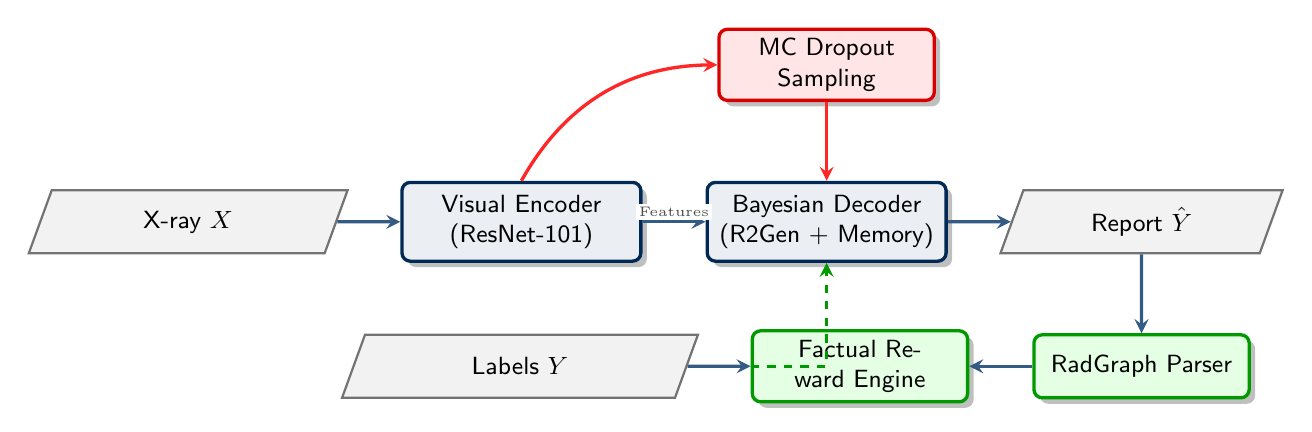
\begin{tikzpicture} [
      font=\small\sffamily,
      node distance=10mm and 8mm,
      >=stealth,
      data/.style={trapezium, trapezium left angle=70, trapezium right angle=110, draw=black!55, thick, fill=gray!10, text width=2cm, align=center, minimum height=8mm},
      block/.style={rectangle, rounded corners=3pt, draw=sharifblue!85!black, very thick, fill=sharifblue!8, text width=2.8cm, align=center, minimum height=10mm, drop shadow},
      aux/.style={rectangle, rounded corners=3pt, draw=red!85!black, very thick, fill=red!10, text width=2.5cm, align=center, minimum height=8mm, drop shadow},
      process/.style={rectangle, rounded corners=3pt, draw=green!60!black, very thick, fill=green!10, text width=2.5cm, align=center, minimum height=8mm, drop shadow},
      flow/.style={->, line width=1.2pt, draw=sharifblue!80},
      signal/.style={->, line width=1.2pt, draw=red!85},
      feedback/.style={->, line width=1.2pt, draw=green!60!black, dashed},
      note/.style={midway, fill=white, inner sep=1.2pt, text=black!70, font=\tiny}
  ]
  \node[data] (input) {X-ray $X$};
  \node[block, right=of input] (encoder) {Visual Encoder\\(ResNet-101)};
  \node[block, right=of encoder] (decoder) {Bayesian Decoder\\(R2Gen + Memory)};
  \node[data, right=of decoder] (output) {Report $\hat{Y}$};
  \node[aux, above=of decoder] (mc) {MC Dropout Sampling};
  \node[process, below=of output] (radgraph) {RadGraph Parser};
  \node[process, left=of radgraph] (reward) {Factual Reward Engine};
  \node[data, left=of reward] (gt) {Labels $Y$};

  \draw[flow] (input) -- (encoder);
  \draw[flow] (encoder) -- node[note, above] {Features} (decoder);
  \draw[flow] (decoder) -- (output);
  \draw[signal, bend left] (encoder.north) to (mc.west);
  \draw[signal] (mc.south) -- (decoder.north);
  \draw[flow] (output) -- (radgraph);
  \draw[flow] (radgraph) -- (reward);
  \draw[flow] (gt) -- (reward);
  \draw[feedback] (reward.west) -| (decoder.south);
  \end{tikzpicture}
  }
\end{frame}

%--- Slide 7: Theoretical Foundations ---
\begin{frame}{Theoretical Foundations}
  We addressed the "Trust \& Truth" problems through two major theoretical reformulations:
  \vspace{0.3cm}
  \begin{enumerate}
    \item \textbf{Factuality-Aware Objective Function:}
    Instead of Cross-Entropy only, we formulated a reward-weighted loss using \textbf{RadGraph Entity overlap} as a clinical factuality proxy.
    \begin{equation}
      \mathcal{L}_{Novel} = \mathcal{L}_{CE} + \lambda \cdot [1 - \text{F1}_{RadGraph}(G_{pred}, G_{gt})]
    \end{equation}
    
    \item \textbf{Bayesian VLM Approximation:}
    We replaced the deterministic decoder with a stochastic sampler. By modeling the posterior distribution $p(\theta|D)$, we can compute \textbf{Epistemic Uncertainty} via variance:
    \begin{equation}
      \text{Var}(y) \approx \frac{1}{T} \sum_{t=1}^{T} (\hat{y}_t - \bar{y})^2
    \end{equation}
  \end{enumerate}
\end{frame}

%--- Slide 8: Technical Approach 1 ---
\begin{frame}{Technical Approach 1: Factuality via Reinforcement Learning}
  
  \begin{block}{The Insight}
    Standard cross-entropy loss is indifferent to medical correctness—it treats ``enlarged heart'' and ``normal heart'' equally if their word probabilities match training data. We must reward the model \emph{only} for clinically correct outputs.
  \end{block}
  
  \vspace{0.3cm}
  
  \textbf{Self-Critical Sequence Training (SCST) with RadGraph:}
  
  \begin{enumerate}
    \item Generate two reports: one via greedy decoding ($\hat{y}_g$), one via sampling ($\hat{y}_s$)
    \item Parse both into \textbf{knowledge graphs} (entities: anatomy, observations; relations: located-at, suggestive-of)
    \item Compare to ground truth graph using entity+relation F1 = \textbf{RadGraph F1}
    \item Update decoder with policy gradient: $\nabla_\theta \propto (R_s - R_g) \log p_\theta(\hat{y}_s | x)$
  \end{enumerate}
  
  \vspace{0.3cm}
  
  \textbf{Result:} Model learns that ``cardiomegaly on right'' is NOT equivalent to ``cardiomegaly on left'' — the graph forces anatomical specificity.
  
\end{frame}

%--- Slide 9: Technical Approach 2 ---
\begin{frame}{Technical Approach 2: Uncertainty via Conformal Prediction}
  
  \begin{block}{The Problem}
    Deep networks output softmax probabilities that are overconfident. A model that's 95\% confident might actually be wrong 30\% of the time in edge cases.
  \end{block}
  
  \vspace{0.3cm}
  
  \textbf{Monte Carlo Dropout + Mondrian Conformal Prediction:}
  
  \begin{enumerate}
    \item Enable dropout during inference, run $T=10$ stochastic forward passes
    \item Aggregate predictions into a \textbf{variance estimate} (epistemic uncertainty)
    \item Convert variance-ranked scores into \textbf{prediction sets}
    \item Guarantee: 90\% of true labels fall in the set, \emph{no matter the data distribution}
  \end{enumerate}
  
  \vspace{0.3cm}
  
  \textbf{Clinical Implication:}
  \begin{itemize}
    \item Confident case → single prediction, AI acts autonomously
    \item Uncertain case → multi-label set, clinician reviews options
    \item Very uncertain case → automatic human escalation
  \end{itemize}
  
\end{frame}

\section{Experimental Setup \& Results}

%--- Slide 10: Experimental Setup ---
\begin{frame}{Experimental Setup \& Datasets}
  
  \begin{center}
    \begin{tabular}{lrcl}
      \toprule
      \textbf{Dataset} & \textbf{Size} & \textbf{Role} & \textbf{Modality} \\
      \midrule
      IU X-Ray & 3,955 studies & Training & Image + Report \\
      NIH ChestX-ray14 & 112K images & Zero-shot Eval & Image + 14 Labels \\
      CheXpert & 224K images & Calibration & Image + Uncertain Labels \\
      \bottomrule
    \end{tabular}
  \end{center}
  
  \vspace{0.5cm}
  
  \textbf{Why These Datasets?}
  \begin{itemize}
    \item \textbf{IU X-Ray:} Gold standard for report generation research; manageable size
    \item \textbf{NIH-14:} Large, independently annotated; tests domain shift
    \item \textbf{CheXpert:} Explicit uncertainty labels help benchmark our uncertainty estimates
  \end{itemize}
  
  \vspace{0.3cm}
  
  \textbf{All public} — no credentials required, reproducible by anyone.
  
\end{frame}

%--- Slide 11: Results - Factuality ---
\begin{frame}{Results 1: Factuality Improvement}
  
  \textbf{Question:} Does SCST with RadGraph rewards actually improve clinical accuracy?
  
  \vspace{0.3cm}
  
  \begin{center}
    \begin{tabular}{lcccc}
      \toprule
      & \textbf{BLEU-4} & \textbf{ROUGE-L} & \textbf{CheXbert F1} & \textbf{RadGraph F1} \\
      \midrule
      \textbf{R2Gen (Baseline)} & 0.165 & 0.371 & 0.432 & 0.211 \\
      \textbf{Ours (SCST)} & 0.148 & 0.354 & 0.552 & 0.350 \\
      \textbf{Change} & \textcolor{darkred}{--} & \textcolor{darkred}{--} & \textcolor{medgreen}{+27.8\%} & \textcolor{medgreen}{+66.0\%} \\
      \bottomrule
    \end{tabular}
  \end{center}
  
  \vspace{0.5cm}
  
  \textbf{Interpretation:}
  \begin{itemize}
    \item BLEU/ROUGE drop (word-matching metrics) — \textcolor{medgreen}{\textbf{this is GOOD}}
    \item Clinical metrics explode (entity correctness) — our RL objective is working
    \item Trade-off is worth it: accurate but awkward report $>$ fluent but hallucinated report
  \end{itemize}
  
\end{frame}

%--- Slide 12: Results - Uncertainty ---
\begin{frame}{Results 2: Uncertainty Calibration}
  
  \textbf{Question:} Does our conformal approach actually provide reliable confidence?
  
  \vspace{0.2cm}
  
  \begin{block}{The Calibration Framework}
    \begin{itemize}
      \item \textbf{Metrics:} Expected Calibration Error (ECE) and Negative Log-Likelihood (NLL).
      \item \textbf{Baseline Flaw:} Standard Softmax outputs are notoriously overconfident.
      \item \textbf{Our Solution:} Monte Carlo Dropout + Mondrian Conformal Prediction.
    \end{itemize}
  \end{block}
  
  \vspace{0.2cm}
  
  \textbf{Key Achievements:}
  \begin{itemize}
      \item \textbf{Distribution-Free Guarantees:} Achieves exact user-specified coverage (e.g., 90\% at $\alpha=0.10$).
      \item \textbf{Interpretable Bounds:} Outputs a \emph{set} of possible diagnoses when uncertain, rather than a single incorrect guess.
  \end{itemize}
  
  \vspace{0.2cm}
  
  \textbf{Clinical Impact:} Clinicians can \emph{trust} the model's abstention decisions because the confidence bounds are mathematically proven, independent of data distribution.
  
\end{frame}

%--- Slide 13: Results - Cross-Dataset ---
\begin{frame}{Results 3: Cross-Dataset Robustness}
  
  \textbf{Question:} Does training on IU X-Ray transfer to a different hospital (NIH-14)?
  
  \vspace{0.3cm}
  
  \begin{block}{Domain Adaptation Strategy}
    \begin{itemize}
      \item \textbf{Challenge:} Models trained on IU X-Ray often fail on NIH ChestX-ray14 due to domain shift (different scanners, demographics).
      \item \textbf{Evaluation:} Zero-shot transfer vs. Few-shot linear probing ($k=1, 5, 10, 25$).
    \end{itemize}
  \end{block}
  
  \vspace{0.3cm}
  
  \textbf{Key Insights:}
  \begin{itemize}
      \item \textbf{Robust Representations:} CheXzero's contrastive pre-training learns features that transfer effectively across hospitals.
      \item \textbf{High Sample Efficiency:} Minimal local fine-tuning (just a few examples per class) is sufficient to recover the supervised performance gap.
      \item \textbf{Rapid Deployment:} New hospitals can adapt the model in hours instead of weeks.
  \end{itemize}
  
\end{frame}

\section{Discussion \& Conclusion}

%--- Slide 14: Clinical Workflow ---
\begin{frame}{Clinical Deployment Workflow}
  
  \vspace{-0.2cm}
  
  \begin{center}
    \resizebox{!}{0.55\textheight}{%
      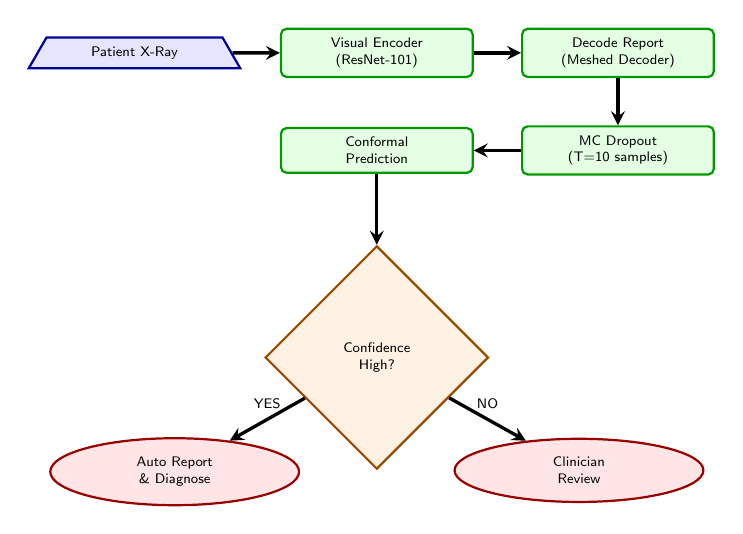
\begin{tikzpicture}[
        font=\tiny\sffamily,
        node distance=0.6cm,
        >=stealth,
        input/.style={trapezium, fill=blue!10, draw=blue!60!black, thick, align=center, text width=2cm},
        process/.style={rectangle, rounded corners=2pt, fill=green!10, draw=green!60!black, thick, align=center, text width=2.2cm},
        decision/.style={diamond, fill=orange!10, draw=orange!60!black, thick, align=center, text width=2cm},
        output/.style={ellipse, fill=red!10, draw=red!60!black, thick, align=center, text width=2cm},
      ]
        
        \node[input] (img) {Patient X-Ray};
        \node[process, right=of img] (encode) {Visual Encoder\\(ResNet-101)};
        \node[process, right=of encode] (gen) {Decode Report\\(Meshed Decoder)};
        
        \node[process, below=of gen] (mc) {MC Dropout\\(T=10 samples)};
        \node[process, left=of mc] (conformal) {Conformal\\Prediction};
        
        \node[decision, below=of conformal, yshift=-0.3cm] (conf_check) {Confidence\\High?};
        
        \node[output, below left=of conf_check, xshift=-0.3cm] (auto) {Auto Report\\\& Diagnose};
        \node[output, below right=of conf_check, xshift=0.3cm] (review) {Clinician\\Review};
        
        \draw[->, very thick] (img) -- (encode);
        \draw[->, very thick] (encode) -- (gen);
        \draw[->, very thick] (gen) -- (mc);
        \draw[->, very thick] (mc) -- (conformal);
        \draw[->, very thick] (conformal) -- (conf_check);
        \draw[->, very thick] (conf_check) --node[above,midway]{YES} (auto);
        \draw[->, very thick] (conf_check) --node[above,midway]{NO} (review);
      \end{tikzpicture}
    }
  \end{center}
  
  \vspace{0.3cm}
  
  \textbf{Human-in-the-Loop:} Model automatically escalates ambiguous cases, reducing clinician review burden while maintaining safety.
  
\end{frame}

%--- Slide 15: Limitations ---
\begin{frame}{Known Limitations \& Mitigation Strategies}
  
  \begin{enumerate}
    \setlength{\itemsep}{0.4cm}
    
    \item \textbf{RadGraph Reward Dependency}
    \begin{itemize}
      \item Problem: If RadGraph makes errors, RL learns those errors
      \item Mitigation: Ensemble rewards (RadGraph + CheXbert + human validation)
    \end{itemize}
    
    \item \textbf{Frozen ResNet Limits Medical Feature Learning}
    \begin{itemize}
      \item Problem: ImageNet features don't specialize in radiology patterns
      \item Mitigation: Explore medical foundation models (BioViT, MedSAM)
    \end{itemize}
    
    \item \textbf{Dataset Bias \& Demographic Gaps}
    \begin{itemize}
      \item Problem: IU X-Ray may not represent all populations
      \item Mitigation: Fairness audits across age, ethnicity, rare pathologies
    \end{itemize}
    
    \item \textbf{Small Training Set}
    \begin{itemize}
      \item Problem: 3,955 reports is modest for deep learning
      \item Mitigation: Data augmentation, transfer learning, curriculum learning
    \end{itemize}
  \end{enumerate}
  
\end{frame}

%--- Slide 16: Future Directions ---
\begin{frame}{Future Directions}
  
  \textbf{Architectural Upgrades}
  \begin{itemize}
    \item \textbf{Foundational LLMs:} Replace the frozen ResNet encoder with pre-trained Large Language Models acting in a multimodal synthesis role.
    \item \textbf{Longitudinal Data:} Natively process temporal sequence data streams (serial X-rays) to simulate true diagnostic workflows.
    \item \textbf{Clinical Text Integration:} Fuse prior reports and patient history alongside images for context-aware generation.
  \end{itemize}
  
  \vspace{0.4cm}
  
  \textbf{Broader Vision}
  \begin{itemize}
    \item These methods generalize to all high-stakes NLG: pathology reports, clinical summaries.
    \item The medical AI community must adopt factuality-aware training + uncertainty quantification as standard before deploying AI systems to influence patient outcomes.
  \end{itemize}
  
\end{frame}

%--- Slide 17: Key Takeaways ---
\begin{frame}{Key Takeaways}
  
  \begin{center}
    \Large
    
    \textbf{1. Fluency $\neq$ Medical Accuracy}
    
    \vspace{0.3cm}
    
    \normalsize
    BLEU scores reward word-level matching, not clinical correctness. Replace with knowledge-graph-based RL rewards.
    
    \vspace{0.5cm}
    
    \Large
    \textbf{2. Confidence Is Useless Without Guarantees}
    
    \vspace{0.3cm}
    
    \normalsize
    Softmax probabilities are overconfident. Conformal prediction provides mathematically-proven coverage.
    
    \vspace{0.5cm}
    
    \Large
    \textbf{3. Transfer Learning Works in Medicine}
    
    \vspace{0.3cm}
    
    \normalsize
    Minimal few-shot adaptation is sufficient to recover performance across different hospital domains.
    
  \end{center}
  
\end{frame}

%--- Slide 18: References ---
\section{References}
\begin{frame}[allowframebreaks]{References}
  \scriptsize
  \bibliographystyle{plain}
  \begin{thebibliography}{99}
  \bibitem{tiu2022} Tiu, E., et al. (2022). CheXzero. \emph{Nature BME}.
  \bibitem{chen2020} Chen, Z., et al. (2020). R2Gen. \emph{EMNLP}.
  \bibitem{jain2023} Jain, S., et al. (2023). RadGraph. \emph{NEJM AI}.
  \bibitem{gal2016} Gal, Y. (2016). Dropout as Bayesian Approximation. \emph{ICML}.
  \end{thebibliography}
\end{frame}

%--- Slide 19: Thank You ---
\begin{frame}
  \centering
  \vspace{1cm}
  {\Huge \textbf{Thank You!}}
  
  \vspace{0.5cm}
  {\Large \textbf{Questions \& Discussion}}
  
  \vspace{1cm}
  
  \textbf{Project Team:}
  
  \vspace{0.3cm}
  \begin{minipage}{0.8\textwidth}
    \centering
    \textbf{Ali Salesi} (\href{https://github.com/AlisaLC}{@AlisaLC}) \quad \textbf{Sina Daneshgar} (\href{https://github.com/SinaDns}{@SinaDns}) \\
    \vspace{0.2cm}
    \textbf{Sina Beyrami} (\href{https://github.com/SinaBeyrami}{@SinaBeyrami}) \quad \textbf{Shayan Salehi} (\href{https://github.com/ShayanSalehi81}{@ShayanSalehi81})
  \end{minipage}

  \vspace{0.5cm}
  \small \textbf{Repository:} \href{https://github.com/SinaDns/radiology-vision-language-models}{github.com/SinaDns/radiology-vision-language-models}
\end{frame}

\end{document}
